% Note that the text in the [] brackets is the one that will
% appear in the table of contents, whilst the text in the {}
% brackets will appear in the main thesis.

%% CHAPTER HEADER /////////////////////////////////////////////////////////////////////////////////////
\chapter{Numerical Simulation Pre-processing and the Convergence Tests}
\label{ch:simulation}

%% CHAPTER INTRODUCTION ///////////////////////////////////////////////////////////////////////////////
The Chapter presents the sample configuration for numerical simulations based on the \ac{sem}.
The configuration matches the specimen used to validate the model experimentally.
The description contains the overall dimensions of \ac{hsc} panel, sensor placement, the material properties, and the excitation signal.
It is demonstrated how the individual components were meshed to improve computer operations.
Two disbonds models are described in the Chapter.
In the first model, the core cells from the damaged area were removed, and in the second model, the interface components between the adhesive layer and the core were removed from the damaged area.

The end of the Chapter features a presentation of temporal and spatial convergence tests of the implemented models.
The time convergence test showed that while the time step is selected above the critical value it results in immediate displacements to infinity.
On the other hand, the spatial convergence test consisted of selecting the order of the polynomial interpolation of the spectral elements to obtain a convergence error below the assumed threshold.
%% INCLUDE SECTIONS ///////////////////////////////////////////////////////////////////////////////////

%% SECTION HEADER /////////////////////////////////////////////////////////////////////////////////////
\section{Excitation signal}
\label{sec:excitation}

%% SECTION CONTENT ////////////////////////////////////////////////////////////////////////////////////
A sine function modulated by the Hann window was chosen as the excitation signal.
It is defined as:
\begin{eqnarray}
	V_e(t) = 0.5\left(1-\cos(2\pi f_m(t-1/f_m)\right)\sin(2\pi f_ct),
\end{eqnarray}
where \(f_c\) is the carrier frequency, and \(f_m=f_c/N_c\) is the modulation frequency with \(N_c\) as the number of cycles.
\(N_c\) was assumed to be five, as a compromise between signal length in the time domain and signal width in the frequency domain.
It is because too high \(N_c\) may cause overlapping wave modes, while too low number will cause increasing signal dispersion.
Both issues can cause difficulties in signal processing for damage assessment.
The set of carrier frequencies was considered to be \(f_c=[50, 100, 150] \) \unit{\kHz}.

The convergence of the solution of the equation of motion requires time increment to be less than a critical value.
If the increment is adopted too large, the displacements immediately tend towards infinity due to increasing numerical errors.
Therefore, a maximum step value is sought for which the solution is stable. 
In the present models, it is obtained for \(\Delta t=\)\num{12.2e-3} \(\mu\)s, which represents more than 80 \unit{\MHz} of the sampling frequency.

%% SECTION HEADER /////////////////////////////////////////////////////////////////////////////////////
\section{Sample Configuration}
\label{sec:sample}

%% SECTION CONTENT ////////////////////////////////////////////////////////////////////////////////////
The sample of interest was a \(500\times500\times1.5\) mm\(^3\) unidirectional \ac{cfrp} in stack sequence \([0^{\circ},90^{\circ}]_s\) plate bonded to an aluminium honeycomb core. 
It was decided to use only one skin, as it is pictured in Fig.~\ref{fig:honeycomb}(b), with the intention of experimental validation and to be able to enlarge disbonds between the skin and the core located in the middle of the \ac{hsc} with a tool in a real sample. 
It was not decided to dedicate separate samples for each size of damage because too many factors would affect the signal value, including skin and sensors properties, the thickness of the adhesive layers, position of the core relative to the sensors, and distance between sensor.
\begin{figure}[H]
	\begin{center}
		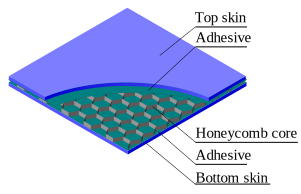
\includegraphics{Chapter_5/honeycomb}
	\end{center}
	\caption{Sample configuration: (\textbf{a}) top view of the sample, (\textbf{b}) honeycomb sandwich substructures and (\textbf{c}) details of the honeycomb cell.}
	\label{fig:honeycomb}
\end{figure}

The core geometry is accurately reproduced from the actual specimen, i.e., incorrect hexagonal \(\left(\mathrm{h}_1 \ne \mathrm{l}_1\right)\) and double walls at the sheet joints, resulting from the core fabrication technology.
According to the drawing in Fig.~\ref{fig:honeycomb}(\textbf{c}), the cell dimensions are w=0.1 mm, h\(_1\)=11 mm, h\(_2\)=5 mm, l\(_1\)=10.4 mm, l\(_2\)=6 mm and the cell height g=14.5 mm.
The core was bonded to one \ac{cfrp} plate using the epoxy adhesive (Loctite EA3479B) with the thickness h\(_a\)=0.3 mm.
The adhesive layer covered the entire bottom surface of the skin.

Signal excitation and recording were accomplished with a pair of \acp{pzt}  (Noliac, NCE51)mounted to the top surface of the skin with cyanoacrylate glue.
The circular transducers of diameter \(\Phi_{PZT}\)=10 mm and thickness h\(_{PZT}\)=0.5 mm were attached 200 mm apart, as shown in Fig.~\ref{fig:honeycomb}(\textbf{a}). The thickness of cyanoacrylate glue under \ac{pzt} was assumed to be h\(_g=50\) \(\mu\)m.

The material properties of the components needed for the simulations are compiled in Tab.~\ref{tab:properties}.
\begin{table}[H]
	\small
	\tabcolsep=0.75cm
	%	\centering
	\caption{\label{tab:properties}The mechanical properties of the materials.}
	\begin{tabular}{ccccc}\toprule
		\multirow{2}{*}{\textbf{Material}} & $\boldsymbol{E_{11}}$ & $\boldsymbol{E_{33}}$ & $\boldsymbol{\nu_{12}}$ & $\boldsymbol{\rho}$ \\ & GPa & GPa & -- & kg/m\(^3\)\\
		\midrule
		Carbon & 275 & 27 & 0.2 & 1900\\
		Epoxy & 3.43 & 3.43 & 0.35 & 1250\\
		Aluminium & 71 & 71 & 0.33 & 2770\\
		Epoxy adhesive & 6 & 6 & 0.34 & 1200\\
		Cyanoacrylate glue & 3 & 3 & 0.34 & 1200\\		
		\bottomrule
	\end{tabular}
\end{table}

%% SECTION HEADER /////////////////////////////////////////////////////////////////////////////////////
\section{GW Propagation in the Real Honeycomb Core Model}
\label{sec:honeycomb}

%% SECTION CONTENT ////////////////////////////////////////////////////////////////////////////////////
All structures used to create the sample were modeled in the simulation with the following elements: 2D for the core, epoxy adhesive and cyanoacrylate glue and 3D for the \ac{cfrp} plate and \acp{pzt}.
During the creation of the mesh, special attention was taken to reduce the number of non-zero values in the matrix \(\textbf{G}\). While the inversion of the matrix \(\left [\textbf{GL}_+^{-1}\textbf{G}^T\right ]\) is necessary to calculate the vector of Lagrange multipliers in \mbox{Equation~(\ref{eq:lambda})} and \(\textbf{L}_+\) is a diagonal matrix, the sparsity of the matrix \(\textbf{G}\) has a significant effect on the computation cost.

One spectral element was intended for each wall of the honeycomb core, while the meshes of the skin plate and the adhesive layer were divided by three rhombus elements per area under the core cell.
In this way, the interface nodes coincide with the nodes lying on the hexagon edges (red line on Figure~\ref{fig:skin_mesh}(\textbf{b})).

The mesh for the cyanoacrylate adhesive consisted of five elements, with a second-order curve at the structure boundary as it is presented in Fig.~\ref{fig:skin_mesh}(\textbf{c}).
This mesh was connected to the the skin with the non-matching interface elements.
The \ac{pzt} mesh coincides with the glue mesh and they are connected with the matching interface elements.
\begin{figure}[H]
	\begin{center}
		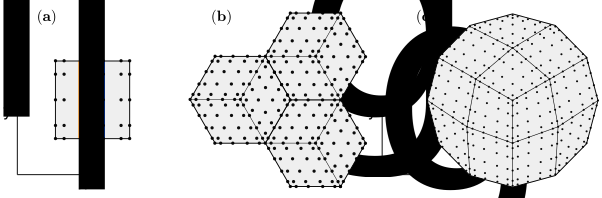
\includegraphics{Chapter_5/skin_mesh}
	\end{center}
	\caption{The mesh with the node distribution, (\textbf{a}) spectral element used for modeling the wall of the core, (\textbf{b}) excerpt of the skin plate and (\textbf{c}) cyanoacrylate glue mesh with the second-order curve at the boundary.}
	\label{fig:skin_mesh}
\end{figure}

The convergence of the solution requires time increment to be less than a critical value, above which the displacements go to infinity.
In the present model, convergence was achieved for \(\Delta t=\)\num{12.2e-3} \(\mu\)s.
The number of nodes for the particular elements are as follows: the core \(6 \times 5\), epoxy adhesive and cyanoacrylate glue \(6 \times 6\), the plate \(6 \times 6 \times 4\) and \acp{pzt} \(6 \times 6 \times 3\).
While the max length of the skin element is six mm, such a \ac{cfrp} model satisfies the condition of at least six nodes per wavelength for the \ac{a0}, as it is the shortest mode propagating in the assumed frequency range.
Table~\ref{tab:wavelength} shows the \ac{a0} wavelengths for various frequency and propagation angles.
\begin{table}[H]
	\small
	\tabcolsep=0.75cm
	%\centering
	\caption{\label{tab:wavelength}The wavelength of the \ac{a0} mode propagated in the presented \ac{cfrp} plate.}
	\begin{tabular}{cccccc}
		\toprule
		\textbf{Frequency} & \multicolumn{5}{c}{\textbf{Propagation angle}}\\
		kHz & \(0^{\circ}\) & \(30^{\circ}\) & \(45^{\circ}\) & \(60^{\circ}\) & \(90^{\circ}\)\\
		\midrule
		50 & 16.5& 15.2&15.0&15.2&16.6\\
		100 & 10.3& 9.6&9.5&9.6&10.3\\
		150 & 7.5& 7.1&7.0&7.1&7.5\\
		\bottomrule
		\multicolumn{6}{r}{{\scriptsize{source: Dispersion Calculator v1.9}}}
	\end{tabular}
\end{table}
%% SECTION HEADER /////////////////////////////////////////////////////////////////////////////////////
\section{\Acf{hcgm}}
\label{sec:homogenised}

%% SECTION CONTENT ////////////////////////////////////////////////////////////////////////////////////
In the section \ref{sec:modelling}, several examples are given of the successful application of the model to numerical analysis of \ac{gw} propagation and damage localisation in \ac{hsc}.
Its unquestionable advantage is the simplified component mesh, reducing operating memory resources.
In dissertation, comparative studies between the \ac{hcgm} and the \ac{fcgm} was conducted to assess the simplified model effectiveness in estimating damage size.

In the \ac{hcgm}, the values of the material constants of the panel core were calculated according to the method presented by Malek and Gibson \cite{malek2015effective}.
This model is an extension of the theoretical analysis of Gibson et al. \cite{gibson1982mechanics}, considering the different geometry of the cell and the nodes at the intersection of the vertical and inclined walls.

The comprehensive formulation of the stiffness matrix components is given in App.~\ref{app:eff_properties} and the effective mechanical properties are gathered in Table \ref{tab:properties_eff}.
The properties for other structures, i.e., the skin, the epoxy adhesive, the cyanoacrylate glue, and the sensors remained unchanged.
The core element has \(6 \times 6 \times 4\) nodes, and the mesh coincides with the skin mesh.
The elements of the other structures are the same as described in the previous section.
%% SECTION HEADER /////////////////////////////////////////////////////////////////////////////////////
\section{Damaged structure implementation}
\label{sec:disbond}
%% SECTION CONTENT ////////////////////////////////////////////////////////////////////////////////////
The skin and the core disbonds were evaluated to analyse the effect of damage on GW propagation.
A rectangular region of disbonds was investigated with the length along the wave propagation varying in width \(\mathrm{w_d} = [0,10,30,50,70,100,120]\) mm, and the damage length in the perpendicular direction was constant \(\mathrm{l_d} = 170\) mm.
The rectangle was centrally located between the transducers, as presented in Figure~\ref{fig:honeycomb}(\textbf{a}).
The selected dimensions of the defects correspond to the dimensions of disbonds made in the specimen to be measured experimentally.
The damage was done with a sharp hooked tool that detached the core from the adhesive layer cell by cell.
The dimensions of the disbond had a coarse tolerance, measuring the width by a calliper.
Due to the small aluminium sheet thickness, the core cells were squashed within the damaged area as it can be seen in Figure~\ref{fig:disbond}\textbf{(a)}.

Two kinds of disbond models were considered in the analysis.
The core cells were removed from the damaged area in the first model as in the mesh pictured in Figure~\ref{fig:disbond}(\textbf{b}).
Whereas in the second model, all components were intact, and only the interface elements between the adhesive layer and the core were decoupled within the yellow area indicated in Figure~\ref{fig:disbond}(\textbf{c}).
\begin{figure}[!bh]
	\begin{center}
		\includegraphics[width=0.9\textwidth]{Chapter_5/disbond}
	\end{center}
	\caption{The damaged area in the: (\textbf{a}) experimental sample,(\textbf{b}) numerical model with removed cells and (\textbf{c}) numerical model with interface decoupling}
	\label{fig:disbond}
\end{figure}
%% SECTION HEADER /////////////////////////////////////////////////////////////////////////////////////
\section{Convergence tests of the solution}
\label{sec:convergence}

%% SECTION CONTENT ////////////////////////////////////////////////////////////////////////////////////

\subsection{Spatial convergence}
Spatial convergence was determined after simulations for samples with elements of different order of the Legendre polynomial (see Eq. \ref{eq:nodes}).
The polynomial order for the \(\xi\times \eta\) plane in the local reference system were changed in the set: \(p=[4,\,5,\,7,\,9,\, 11]\).
The exact order was assumed for each component to minimise the non-zero value of coupling matrix \(\textbf{G}\).
Due to the perpendicularity of the core elements to the skin, the nodes along the core thickness are fixed to 5.
As a criterion for convergence, the percentage error defined as:
\begin{eqnarray}
	\delta^{\mathrm{conv}} = \frac{\sum{\left(e^{\mathrm{max}}-e^{p}\right)^2}}{\sum{\left(e^{max}\right)^2}} \times 100\%,
	\label{eq:perc_err_conv}
\end{eqnarray}
where \(e^{max}\) and \(e^{p}\) are the signal envelopes for the case with the elements of \(11^{\mathrm{th}}\) polynomial order and the observed case, respectively.
A 5\% threshold was assumed for choosing the degree of the polynomial.
The signal envelope is obtained using the Hilbert transform, which is defined as \cite{staszewski2004health}:
\begin{eqnarray}
	\label{eq:hilbert}
	\hat{x}(t) &=& \frac{1}{\pi}\int_{-\infty}^{+\infty}x(\tau)\frac{1}{t-\tau}\diff\tau,\\
	\label{eq:envelope}
	e(t) &=& \sqrt{x^2(t)+\hat{x}^2(t)}.
\end{eqnarray}
\nomtypeD[e]{\(e(t)\)}{Signal envelope}{}%
\nomtypeR[t]{\(t\)}{Time vector}{}{\unit{\second}}%

The example of the simulated signals of 100 \unit{\kHz} are presented in Fig. \ref{fig:dx_conv}\textbf{(a)}.
It can be seen that despite the good agreement of the wave speed for all cases, the amplitudes converge only for a polynomial of order 7.
Based on the graph showing simulation errors (Fig. \ref{fig:dx_conv}(\textbf{b})), the polynomial of order \(p=7\) was selected for 50 and 100 \unit{\kHz} signals, and order \(p=9\) was selected for the 150 \unit{\kHz} signal.
 
Tab \ref{tab:elements_nodes} contains a complete list of elements with the number of nodes on each axis \(\xi\times \eta \times \zeta\) which were assumed in simulations.
\begin{figure}[H]
	\begin{center}
		\includegraphics[width=0.95\textwidth]{Chapter_5/dx_conv}
	\end{center}
	\caption{Spatial convergence for the sample, \textbf{(a)} the sensor signals of 100 \unit{\kHz} for various number of the in-plane nodes (\(n \times m\)) of the element, \textbf{(b)} percent error for the differ polynomial order}
	\label{fig:dx_conv}
\end{figure}
\begin{table}[H]
	\small
	\tabcolsep=0.5cm
	\centering
	\caption{\label{tab:elements_nodes}The node numbers of the sample components.}
	\begin{tabular}{cccc}
		\toprule
		\multirow{3}{*}{\textbf{Component}} & \multicolumn{3}{c}{\textbf{Number of element nodes}}\\
		& \multicolumn{3}{c}{\(n\times m \times l\)}\\
		& 50 \unit{\kHz} & 100 \unit{\kHz} & 150 \unit{\kHz}\\
		\midrule
		Core & \multicolumn{2}{c}{\numproduct{8 x 5 x 1}} & \numproduct{10 x 5 x 1}\\
		Adhesive layer & \multicolumn{2}{c}{\numproduct{8 x 8 x 1}} & \numproduct{10 x 10 x 1}\\
		Skin & \multicolumn{2}{c}{\numproduct{8 x 8 x 4}} & \numproduct{10 x 10 x 1}\\
		Glue & \multicolumn{2}{c}{\numproduct{8 x 8 x 1}} & \numproduct{10 x 10 x 1}\\
		\ac{pzt} & \multicolumn{2}{c}{\numproduct{8 x 8 x 3}} & \numproduct{10 x 10 x 3}\\
		\bottomrule
	\end{tabular}
\end{table}

While the maximum length of the skin element is 6 \unit{\mm}, such a \ac{cfrp} model satisfies the condition of at least six nodes per wavelength for the \ac{a0}, as it is the shortest mode propagating in the assumed frequency range.
Table~\ref{tab:wavelength} shows the \ac{a0} wavelengths for various frequency and propagation angles.
\begin{table}[H]
	\small
	\tabcolsep=0.75cm
	%\centering
	\caption{\label{tab:wavelength}The wavelength of the \ac{a0} mode propagated in the presented \ac{cfrp} plate.}
	\begin{tabular}{cccccc}
		\toprule
		\textbf{Frequency} & \multicolumn{5}{c}{\textbf{Propagation angle}}\\
		\unit{\kHz} & \ang{0} & \ang{30} & \ang{45} & \ang{60} & \ang{90}\\
		\midrule
		50 & 16.5& 15.2&15.0&15.2&16.6\\
		100 & 10.3& 9.6&9.5&9.6&10.3\\
		\bottomrule
		\multicolumn{6}{r}{{\scriptsize{source: Dispersion Calculator v1.9}}}
	\end{tabular}
\end{table}
\subsection{Temporal convergence}
A temporal convergence test is conducted to select the appropriate time step value.
The critical value of time increment (\(\Delta t_{cr}\)) depends on the mesh size and the wave mode velocity.
If this value is set over (\(\Delta t_{cr}\)), the displacement of the structure will increase to infinity in the initial moments of the simulation as it is presented in Fig. \ref{fig:dt_cr}.
This indicates that the time step have to be further decreased which can be easy implemented for testing of the stability of the method.
\begin{figure}[!tbh]
	\begin{center}
		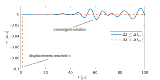
\includegraphics[width=0.95\textwidth]{Chapter_5/dt_cr}
	\end{center}
	\caption{The displacement of the plate at a point of 50 mm away from actuator in the case of correctly and incorrectly selected time increments.}
	\label{fig:dt_cr}
\end{figure}


\section{Conclusions}
\label{sec:conclusionsSimul}

The Chapter describes the whole model configuration for numerical simulations.
The mesh generation for each component, the excitation signals, and the description of damage modelling are included.
A comparison between the \ac{fcgm} and \ac{hcgm} is also provided.

An essential issue in numerical modelling is the convergence of the solution in the spatial and temporal domains.
Incorrectly selected model parameters cause significant errors in the results.
When a time increment is set over the critical value, displacements tend immediately to infinity.
The size and order of the spectral element should be selected depending on the smallest propagating wavelength in the analysed structure.
In turn, the smallest distance between nodes affects the critical value of the time step.
All this has a consequence on the duration of computer simulations.